\documentclass[justified]{tufte-handout}
\usepackage{graphicx,  
            color, 
            subfig, 
            tikz, 
            enumitem, 
            amsmath, 
            relsize,
            listings,
            fancyvrb}
\usepackage[export]{adjustbox}

\hypersetup{colorlinks}

\title{Data Analysis with Python}
\author{Jared Garst}
\date{\today} % remove title space

% itemized list with number and description

\newcommand{\anacondaLink}{https://store.continuum.io/cshop/anaconda/}
\newcommand{\email}{mailto:jgarst@ucdavis.edu}
\newcommand{\aboutUnicodeLink}
  {http://www.joelonsoftware.com/articles/Unicode.html}
\newcommand{\ipythonTutorialLink}
  {http://ipython.org/ipython-doc/stable/interactive/tutorial.html}
\newcommand{\linguaFrancaLink}{http://en.wikipedia.org/wiki/Lingua_franca}
\newcommand{\librariesLink}{http://www.scipy.org/index.html}
\newcommand{\customizeDirectoryLink}
  {http://stackoverflow.com/questions/15680463/change-ipython-working-directory}
\newcommand{\listTutorialLink}
  {https://docs.python.org/2/tutorial/datastructures.html}
\newcommand{\pintLink}{http://pint.readthedocs.org/en/0.6/}
\newcommand{\hgLink}{http://mercurial.selenic.com/}
\newcommand{\gitLink}{http://git-scm.com/}
\newcommand{\lambdaTutorialLink}
  {https://pythonconquerstheuniverse.wordpress.com/2011/08/29/lambda_tutorial/}
\newcommand{\functionalProgrammingLink}
  {http://www.ibm.com/developerworks/library/l-prog/}
\newcommand{\matplotlibGalleryLink}{http://matplotlib.org/gallery.html}

  \newcommand{\myMarginNote}[3][-9px]{\marginnote{\centering{#2} \\ \vspace{#1}
      \justify{#3}}}

  \newcommand{\librariesNote} {\myMarginNote{\href{http://www.scipy.org/index.html}{libraries}}{numpy, scipy,
      matplotlib, and pandas will help you calculate, reference common
      functions, plot, and wrangle data. \texttt{\%matplotlib inline} is a
      'magic function', which tells IPython how to display plots.}}

\newcommand{\cleaningNote} {\myMarginNote{data cleaning}{\texttt{head} and
    \texttt{tail} return the limits of the pandas dataFrame, and are being used
    to check that the csv file doesn't have unexpected cruft at the ends. Always
    check that you are importing your intended data.}}

  \newcommand{\formatNote} {\myMarginNote{\texttt{format}} 
     {adds external variables to strings, at specified precision. 
      \texttt{\{0:.2f\}} is replaced by the first float argument of
      \texttt{format}, rounded to two decimal places.}}

  \newcommand{\argumentNote} {\myMarginNote{argument unpacking}
     {\texttt{function(*iter)} passes the elements of \texttt{itr} to
      \texttt{function} in order. \texttt{function(**dict)} passes them based on
      their keys.}}

  \newcommand{\nonPrimativeNote} {\myMarginNote[-4px]{two types of variables}
    {The copying code produces different results when the strings are not
      wrapped in numpy arrays. Why?}}

  \newcommand{\matplotlibGalleryNote}{\footnote{You will need the syntax for
      matplotlib. You can find everything with the help commands, or can get
      syntax and ideas from \href{\matplotlibGalleryLink}{example plots} that
      others have made.}}

  \newcommand{\floatNote}{\footnote{ Float stands for 'floating
  point number', otherwise known as a decimal number. Though not usually
  relevant for data analysis, be aware that \texttt{int} and \texttt{float} have
  detailed differences in precision and speed.}}

\lstset{showstringspaces=false
        basicstyle=\linespread{.94}\ttfamily,
        fancyvrb=true,
        mathescape=true,
        language=python,
        escapechar=\@
        }


\captionsetup[subfigure]{labelformat=empty, position=top}
\setlength\parindent{0pt}

\newenvironment{absolutelynopagebreak}
  {\par\nobreak\vfil\penalty0\vfilneg
   \vtop\bgroup}
  {\par\xdef\tpd{\the\prevdepth}\egroup
   \prevdepth=\tpd}

\begin{document}
\maketitle
\bigskip

\noindent
Python is a high level scripting language. While there are many reasons to like
or dislike Python, we are introducing it to you because it is becoming the
\href{\linguaFrancaLink}{lingua franca} of
science. This means that increasingly you can expect other people to understand
your code, and for many of your problems to already be solved and documented in
Python. Briefly, some exceptional Python features are:

\begin{description}
\item[Beautiful Syntax] \hfill \\
  Python will make your life easier, by encouraging simple, clean, easy to read
  code.
\item[The Python Shell] \hfill \\
  If you don't need to keep your code, you can pass it to Python as a series of
  commands. This allows programmers to gracefully move their files and explore
  their data.
\item[No Types] \hfill \\
  There is no mechanism to guarantee the data you store will retain important
  properties.
\item[Interpreted] \hfill \\
  The code you write is the code that runs. Nothing will be checked, nothing
  will be optimised.
\item[Program Control Through Indentation] \hfill \\
  Other languages use curly brackets \{\} to determine program flow, and tabs by
  convention for readability. Python conflates the two.
\end{description}

\noindent
IPython is an expansion of the Python shell, designed for a more exploratory
approach to programming than your typical editor. It gives you a unique
structure, and tools to view your output. It also provides you with many tools
that will help you become a better programmer outside this class - we won't get
into many of those, but you can use the standard
\href{\ipythonTutorialLink}{tutorial} to learn them.

\smallskip
\noindent
There are two versions of Python that you will encounter in the wild, Python 2
and Python 3. Python 3 is a take-no-prisoners reimagining of the the
language. The result is a slightly smoother language, that breaks everything
down to the print statement in Python 2. Most libraries support both Python 2
and 3, but most code is in Python 2. This means the appropriate version will
depend on how old your project is. If you are unsure, use Python 2, and consider
that unless you use lots of
\href{\aboutUnicodeLink}{unicode}, switching
to Python 3 will provide only a small benefit to your quality of life.

\section*{Setup and Startup}
If you have never set up a programming environment before, the easiest way to
start is to install \href{\anacondaLink}{Anaconda}, distributed by Continum
Analytics. This modified python environment will install the most common python
libraries. It is distributed for free in hopes of later selling packages that
speed up your python code, but you can simply use it as a convenient
installation tool. If you want to try a grittier, more controlled installation
of Python and its many friends, you can schedule some time with
\href{\email}{Jared}.

\smallskip
\noindent
Once you have completed the installation, run \texttt{ipython notebook} in the
terminal, or the Anaconda IPython Notebook executable. A web browser will
automatically start with your notebook. Managing directories in notebooks is a
little clumsy. Either make sure to run IPython in the directory you want, or
\href{\customizeDirectoryLink}{change the default directory} to match your
workflow.

\smallskip
\noindent
There are a few flavors of help commands available in IPython. Familiarity with
the options allows you to reference the manuals, or explore specific parts of
the language.  \marginnote[25pt]{\centering{A quick start: \\ \texttt{help()} --
    \texttt{help(list)} \\ \texttt{?} -- \texttt{import numpy; numpy?} --
    \texttt{numpy??} \\ \texttt{numpy.*cos*?} -- \texttt{numpy.arc<tab>} --
    \texttt{Ctrl-m h}}}
\\
\begin{description}[font=\tt, leftmargin=0cm]
\item[help()] is the native python help command. Type \texttt{help()} into the
  first cell, and execute with shift-enter. This is a good place to spend time
  getting familiar with the language, but you can also ask it about specific
  objects. For example, run \texttt{help(list)} to see some common list
  manipulations.
\item[?] is IPython's own help command, and it is often nicer to use than
  \texttt{help}. Try running \texttt{?} to see an introduction to IPython. Like
  help you can also ask more specific commands, run \texttt{import numpy;
    numpy?} to see an overview of the exceptionally useful numpy module. If you
  need all the gory details of an object, \texttt{numpy??} will give you the
  source code.
\item[<regex>?] allows you to use \texttt{?} to search through an object. Try
  running \texttt{numpy.*cos*?} to see every function in numpy related to
  $\cos$.
\item[\%quickref] is a 'magic function', unique to IPython, that you can use to
  see a verbatum list of all special IPython commands, including the magic
  functions.
\item[<tab>] will provide code completion. Type but do not run
  \texttt{numpy.arc} followed by a \texttt{<tab>} to have IPython suggest a list
  of inverse trig functions.
\item[Control-m h] Provides a list of hotkeys for IPython notebooks. If you
  spend a lot of time These can
  really speed up your programming,
\end{description}

\pagebreak

\section*{First Steps}
\begin{lstlisting}[language=Python]
  In [1]: import pandas as pd@\librariesNote@
          import numpy as np 
          import matplotlib.pyplot as plt 
          import scipy.stats as st
          %matplotlib inline 
  In [2]: capData = pd.read_csv('DataFile.csv')
          print capData.head()@\cleaningNote@
          print capData.tail()
          @\hfill \texttt{*Some Numbers*}@ 
  In [4]: allData = capData.stack()
          binwidth = 0.2; 
          cmin = capData.min(); 
          cmax = capData.max()
          bins = np.arange(cmin, cmax, binwidth) 
  In [5]: fig, ax = plt.subplots();
          ax.set_xlim([cmin, cmax]);
          ax.hist(list(allData), bins=bins)
  In [6]: N = len(allData) 
          print "N is", N
          mu = np.mean(allData) 
          print "mu is", "{0:.2f}".format(mu) @\formatNote@ 
          var = np.var(allData) 
          print "varience is", "{0:.2f}".format(var) 
          @\hfill \texttt{N is 1536} @
          @\hfill \texttt{mu is 94.50} @
          @\hfill \texttt{variance is 3.02} @
  In [7]: area = N * binwidth 
          params = {'loc':mu, 'scale':np.sqrt(var)} 
          fit = area * st.norm(**params).pdf(bins)@\argumentNote@ 
          ax.plot(bins, fit, 'r--', linewidth=3); 
          fig
          @\vspace{-15px}
          \begin{figure}[h!]
            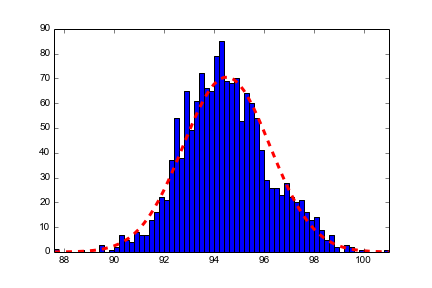
\includegraphics[width=0.63\textwidth, right]{figs/firstPlot.png}
          \end{figure}@


\end{lstlisting}

\section*{Python Gotchas}
Some of the ways that python makes your life easier can send your program off
the rails, if you don't understand what the computer is doing.

\newthought{TYPES} still exist in python, even if you can't enforce
them. Consider the following python code:
\begin{adjustwidth}{2.5em}{0pt}
\begin{lstlisting}[language=Python]
In [1]: print 3/2, 3.0/2.0
@\hfill \texttt{1 1.5}@
\end{lstlisting}
\end{adjustwidth}

\noindent
In the underlying C code, an operation on two integers always returns an
integer, because floating point\floatNote \;math is much slower. In python,
you can check a type with \lstinline !type(!object\lstinline !)!, and enforce a
type with \lstinline !assert! and \lstinline !isinstance!.
\begin{adjustwidth}{2.5em}{0pt}
\begin{lstlisting}[language=Python]
In [2]: print type(3), type(3.0)
@\hfill \texttt{<type 'int'> <type 'float'>}@
In [3]: assert isinstance(3, int)
\end{lstlisting}
\end{adjustwidth}
\lstinline !assert! will stop the program with an error if the next statement is
not true. Python 3 is smarter about division, and will return 1.5 for both
calculations. In the likely event that you cannot use python 3, you can still
import the behavior by including
\begin{adjustwidth}{2.5em}{0pt}
\begin{lstlisting}[language=Python]
from __future__ import division
\end{lstlisting}
\end{adjustwidth}
at the top of your file or notebook.

\newthought{COPYING OBJECTS} can be done in two distinct ways, shown abstractly
in Figure \ref*{fig:copy}. The more common method is to copy the object
reference, so that it can be used in a different part of the code. The second
method is when you want to have two distinct copies, so that you can have both
an original version and a modified version. In the first case it is appropriate
to duplicate the pointer. In the second case it is necessary to duplicate the
object itself.


\smallskip
\begin{marginfigure}
    \vspace*{\fill}
    \centering
    \subfloat[Case 1]{\scalebox{1}{\definecolor{cffffff}{RGB}{255,255,255}


\begin{tikzpicture}[scale=0.7, y=0.80pt,x=0.80pt,yscale=-1, inner sep=0pt, outer sep=0pt]
\begin{scope}[shift={(-1.0,-0.5)}]
  \path[draw=black,fill=cffffff] (101.0000,41.0000) ellipse (1.1289cm and
    1.1289cm);
  \path[draw=black,miter limit=10.00,line width=1.040pt] (175.4493,153.4493) --
    (137.0800,77.8500);
  \path[draw=black,miter limit=10.00,line width=1.040pt] (26.5507,153.4493) --
    (64.9200,77.8500);
  \path[rounded corners=0.0000cm] (1.0000,111.0000) rectangle (71.0000,131.0000);
  \begin{scope}[shift={(0.39716,153.06265)}]
  \end{scope}
  \path[rounded corners=0.0000cm] (131.0000,111.0000) rectangle
    (201.0000,131.0000);
  \begin{scope}[shift={(150.04249,153.06265)}]
  \end{scope}
  \path[rounded corners=0.0000cm] (81.0000,21.0000) rectangle (121.0000,61.0000);
  \begin{scope}[shift={(83.0,26.0)}]
  \end{scope}
  \path[draw=black,fill=black,miter limit=10.00] (134.6900,73.1800) --
    (141.0000,77.8100) -- (137.0800,77.8500) -- (134.7700,81.0000) -- cycle;
  \path[draw=black,fill=black,miter limit=10.00] (67.3100,73.1800) --
    (61.0000,77.8100) -- (64.9200,77.8500) -- (67.2300,81.0000) -- cycle;
\end{scope}

\end{tikzpicture}
}}
    
    \vfill
    
    \subfloat[Case 2]{\scalebox{0.69}{\definecolor{cffffff}{RGB}{255,255,255}

\begin{tikzpicture}[y=0.80pt,x=0.80pt,yscale=-1, inner sep=0pt, outer sep=0pt]
\begin{scope}[shift={(-12.28125,-0.5)}]
  \path[shift={(47.03197,0)},draw=black,fill=cffffff] (41.0000,41.0000) ellipse
    (1.1289cm and 1.1289cm);
  \path[draw=black,miter limit=10.00,line width=1.040pt] (51.9520,77.8500) --
    (12.8520,154.1800);
  \path[draw=black,fill=black,miter limit=10.00] (54.3420,73.1800) --
    (48.0320,77.8100) -- (51.9520,77.8500) -- (54.2620,81.0000) -- cycle;
  \path[rounded corners=0.0000cm] (68.0320,21.0000) rectangle (108.0320,61.0000);
  \path[draw=black,fill=cffffff] (191.0000,41.0000) ellipse (1.1289cm and
    1.1289cm);
  \path[draw=black,miter limit=10.00,line width=1.040pt] (266.1800,154.1800) --
    (227.0800,77.8500);
  \path[draw=black,fill=black,miter limit=10.00] (224.6900,73.1800) --
    (231.0000,77.8100) -- (227.0800,77.8500) -- (224.7700,81.0000) -- cycle;
  \path[rounded corners=0.0000cm] (171.0000,21.0000) rectangle (211.0000,61.0000);
\end{scope}
\begin{scope}[shift={(-12.78125,-1.0)}]
\end{scope}

\end{tikzpicture}}}
    %\subcaption{Case 2}
  \caption{The finger pointing at the moon is not the moon}
  \label{fig:copy}
\end{marginfigure}

\noindent
Because the first case is common and the second case is expensive, python
duplicates the reference by default.
\begin{adjustwidth}{2.5em}{0pt}
\begin{lstlisting}[language=Python]
In[1]: import numpy as np
In[2]: lst1 = np.array([`An Object'], 
                       dtype=object); 
       lstcpy = lst1; lst2 = lst1.copy()
In[3]: print lst1, lstcpy, lst2 
@\hfill \texttt{[`An Object'] ['An Object'] ['An Object']}@
In[4]: lstcpy[0] = 'A New Object'
In[5]: print lst1, lstcpy, lst2
@\hfill \texttt{['A New Object'] ['A New Object'] ['An Object']}@ @\nonPrimativeNote@
\end{lstlisting}
\end{adjustwidth}


\newthought{THE NOTEBOOK STATE} is changed every time you run a command, not
every time you add a cell. This allows you to create confusing code, by removing
cells or executing them in a strange order.

\begin{adjustwidth}{2.5em}{0pt}
\begin{lstlisting}[language=Python]
In [3]: message = 'IPython does not have to run 
          from top to bottom'
In [1]: message = 'Good luck debugging this'
In [4]: print message
  @\hfill \texttt{IPython does not have to run from top to bottom}@ 
In [2]: print message
  @\hfill \texttt{Good luck debugging this}@
\end{lstlisting}
\end{adjustwidth}

\noindent
You can debug this problem by paying attention to the numbers in front of the
cells. Commands are executed in sequence with their numbers, not their
position. Try to keep your notebook linear, by not changing cells that have
already successfully executed.
%\section*{Nuts and Bolts}
%;
%
%referencing input/output In[n], \_i, Out[n], \_ \%reset
%
%\%history
%
%using !, using \$, \{\}
%
%\%\%

\section*{Problems}
\vspace{-0.5cm}

\begin{itemize}
\item[] \newthought{{\Large 1} \hspace{0.25em} DOCUMENTATION FROM PYTHON} \\
  Use the help commands to locate the \texttt{scipy.stats} documentation on the
  Poisson distribution. Is the distribution a function or an object?
  Plot\matplotlibGalleryNote \;the expected number of counts for 10 trials of a
  poisson process, each with an average of 3 counts per trial.

\item[] \newthought{{\Large 2} \hspace{0.25em} DOCUMENTATION FROM GOOGLE} \\
  Try calling the poisson distribution function from \texttt{scipy.stats} with
  no arguments. You will get an error message saying one argument was passed,
  but two were needed. Use google to explain these strange parameter counts.

\item[] \newthought{{\Large 3} \hspace{0.25em} USING PYTHON TO CALCULATE} \\
  Reproduce the mean, variance, and standard deviation of the data using your
  own functions.

  % \item The $\chi^2$ for a frequency distribution is traditionally taken to
  %   be $$ \mathlarger{\mathlarger{\sum}} \; \frac{\left( \text{observed} -
  %     \text{expected}\right)^2}{\text{expected}}$$

  %   How does this compare to a $\chi^2$ test with the points have errors
  %   associated with them? \\
  %   What distribution would you use to make the two equivalent?

%\item 

\item[] 
\newthought{{\Large 4} \hspace{0.25em} OBSERVE THE CENTRAL LIMIT THEOREM} \\
  Write a function \texttt{dataAvg(list, n)} that returns a new list
  $\bar{x}_n$, containing all possible averages of n values from
  \texttt{list}. Use this to plot $\bar{x}_2$, $\bar{x}_{10}$ and
  $\bar{x}_{100}$. What are the means of these averaged distributions? What are
  the variances? How do these compare to the mean and variance of $x$?
\end{itemize}

%\section*{Vocabulary}
%\begin{description}
%\item Types \hfill \\
%  At the lowest level, your computer only works with numbers of finite size,
%  which it can use to reference every color, character or process you might
%  need to use. One of the first advances in programming was assigning 'types'
%  to these numbers, so that your computer will

%\item Object \hfill \\
%Every piece of information your program tracks is not independent

%\end{description}

\pagebreak

\section*{More Reading}
\begin{description}
\item \href{\listTutorialLink}{Data Structures and List Maniupulation}

\item \href{\pintLink}{Units and Errors}

\item Source control: \href{\hgLink}{Mercurial} and \href{\gitLink}{Git}

\item \href{\lambdaTutorialLink}{Lambda Functions} and
  \href{\functionalProgrammingLink}{Functional programming}

\end{description}
\end{document}

